\documentclass[10pt,a4paper,titlepage]{report}
\usepackage[utf8]{inputenc}
\usepackage{amsmath}
\usepackage{amsfonts}
\usepackage{listings}
\usepackage{amssymb}
\usepackage{graphicx}
\usepackage{xcolor}
\usepackage[cache=false]{minted}

\nonstopmode

\begin{document}

{\fontfamily{cmr}\selectfont
\title{ \normalsize \textsc{}
\\ [2.0cm]
\hrulefill \\
\LARGE \textbf{\uppercase{installation of postgresql}\\
\hrulefill \\ [0.5cm]
\normalsize \today \vspace*{5\baselineskip}}
}

\date{}

\author{
	Rwithik Manoj \\ 
	College of Engineering, Trivandrum \\
	Department of Computer Science and Engineering }

\maketitle
\tableofcontents
\newpage

\sectionfont{\scshape}

\chapter{Installation}

\begin{enumerate}
	\item Install the postgresql package. It will also create a system user called postgres. 
		\begin{verbatim}
$ sudo pacman -S postgresql
		\end{verbatim}
		
\includegraphics[width=\linewidth]{../Images/Installation/1.png}\newline
		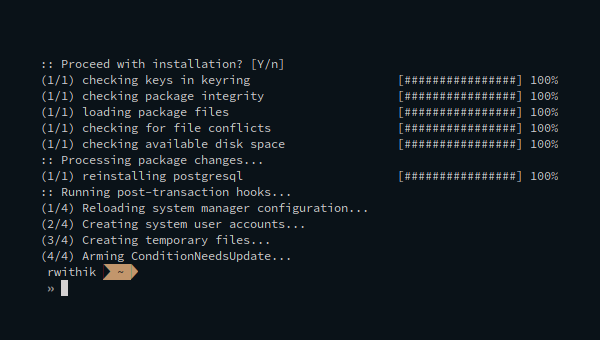
\includegraphics[width=\linewidth]{../Images/Installation/2.png}\newline
		\item You can switch to the PostgreSQL user by executing the following command:
		\begin{verbatim}
$ sudo -iu postgres
		\end{verbatim}
\end{enumerate}

\chapter{Initial Configuration}

\begin{enumerate}
	\item A database cluster must be initialized before \mintinline{psql}{postgres} can be used. Execute the following command as the postgres user:
	\begin{verbatim}
$ initdb -D /var/lib/postgres/data
	\end{verbatim}
	where -D option gives the location of the database cluster.
	Other optional arguments include:
		\begin{verbatim}
	    --locale=locale, where locale is to be chosen amongst the 
				system's available locales
		    -E encoding for the encoding (which must match the chosen locale);
		\end{verbatim}
		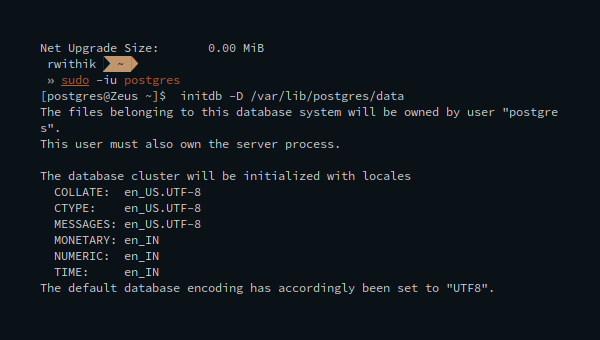
\includegraphics[width=\linewidth]{../Images/Installation/3.png}\newline
		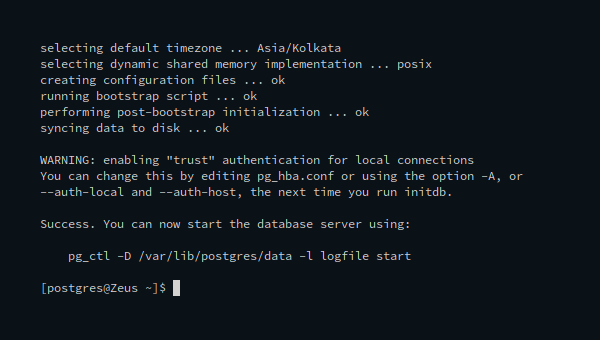
\includegraphics[width=\linewidth]{../Images/Installation/4.png}\newline
	\item Start and enable \verb-postgresql.service-. 
		\begin{verbatim}
		$ sudo systemctl start postgesql.service
		$ sudo systemtcl enable postgresql.service
		\end{verbatim}
		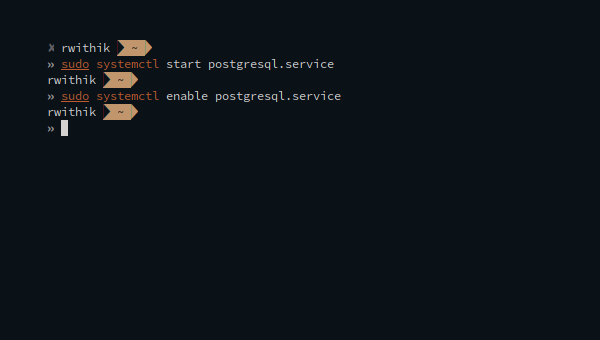
\includegraphics[width=\linewidth]{../Images/Installation/5.png}\newline
	\item Create a new database user. Execute this command as the \verb-postgres- user:
			\begin{verbatim}
			$ createuser --interactive
			\end{verbatim}
	\item Create a new database. Run this command as the regular user:
			\begin{verbatim}
			$ createdb myDatabaseName
			\end{verbatim}
		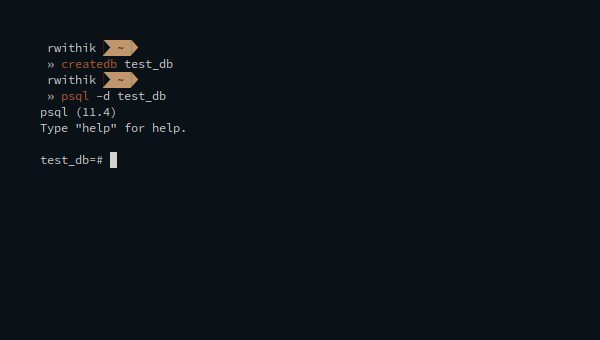
\includegraphics[width=\linewidth]{../Images/Installation/6.png}\newline
				
\end{enumerate}


}
\end{document}
